\documentclass[11pt]{article}
\usepackage[parfill]{parskip}
\usepackage{graphicx}
\usepackage{wrapfig}
\usepackage[top=1in, bottom=1in, left=1in, right=1in]{geometry}
\bibliographystyle{plain}
\usepackage{amsmath}
\usepackage{hyperref}
%%%%%%%%%%%%%%%%%%%%%%%%%%%%%%%%%%%%%%%%%%%%%%%%%%%%%%%%%%%%%%%
\usepackage{fancyhdr}
\pagestyle{fancy}
%%% Please add the author's last names
\lhead{Borlaug, Hodgkin and Shannon}
\rhead{Modeling the World's Systems, 2019}
%%% Please use \cfoot{} to remove page numbers
\cfoot{No page numbers! See latex source.}
\renewcommand{\headrulewidth}{0pt}
\renewcommand{\footrulewidth}{0pt}
%%%%%%%%%%%%%%%%%%%%%%%%%%%%%%%%%%%%%%%%%%%%%%%%%%%%%%%%%%%%%%&
\usepackage{titlesec}
\titlespacing{\section}{0pt}{\parskip}{-.5\parskip}
\titlespacing{\subsection}{0pt}{\parskip}{- .5\parskip}
\titlespacing{\subsubsection}{0pt}{\parskip}{- .5\parskip}
\newcommand{\closeup}{\setlength{\itemsep}{-4pt}}

\date{\vspace{-5ex}}
% Use this to get rid of the date

\usepackage{authblk}
\author[1]{Eric Davis}
\author[1]{Alec Theriault}
\author[1]{Max Orhai}
\author[1]{Eddy Westbrook}
\author[1]{Ryan Wright}
\affil[1]{Galois, Inc}

%\setcounter{page}{0}



\title{Machine-Assisted Extraction of Formal Semantics from Domain Specific Semi-Formal Diagrams}

\begin{document}
\maketitle
\vspace{10pt}
\begin{abstract}
Please keep your abstract short, fifteen lines or less.  Remember that the MWS conference is attended by people from many academic disciplines, as well as colleagues in government, industry, foundations and nonprofits, and the defense and intelligence communities.  So strive to make your abstract accessible.
\end{abstract}

\section{Introduction}

\begin{wrapfigure}{r}{0.5\textwidth}
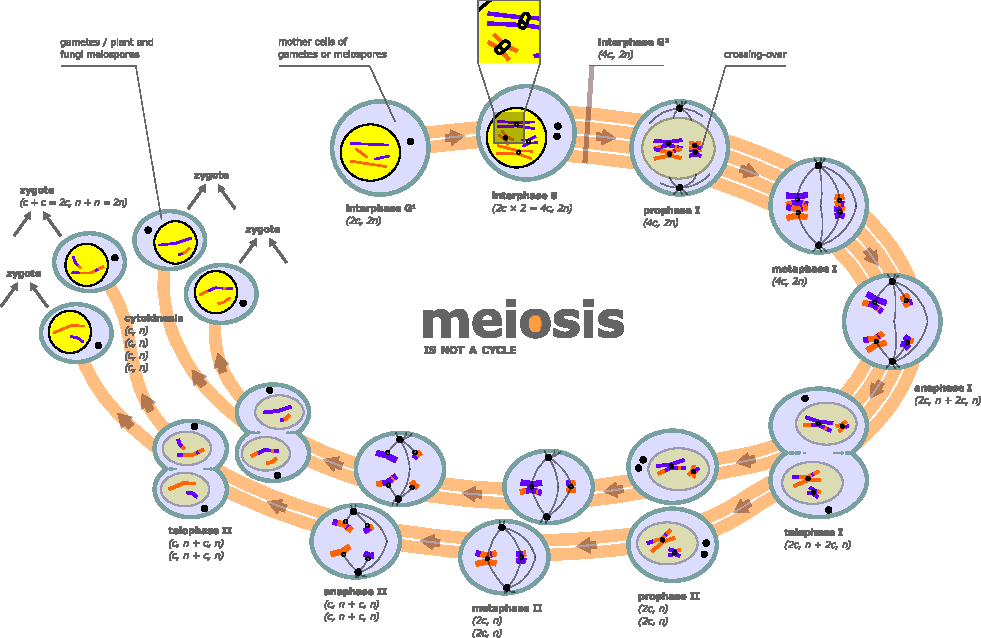
\includegraphics[width=0.48\textwidth]{figs/Diagram_of_meiosis.pdf}
\caption{Example of a semi-formal diagram of Meoisis.\protect\footnotemark}
\label{Fig:Meiosis}
\end{wrapfigure}

\footnotetext{CC-BY-SA 3.0 Marek Kultys, July 2, 2008.}

\paragraph{Significance}

\section{Related Work}

\subsection{Generating Formal Meaning from Informal Diagrams}

\section{AMIDOL}

\subsection{Visual Domain Specific Languages}

\subsection{Intermediate Representation}

\subsection{Inference Engine}

\section{Compartmental Model for Epidemiology}

\subsection{SIRS Model}

H1N1 $R_0$ importance \cite{fraser2009pandemic}.

Ebola $R_0$ importance \cite{fisman2014early}

CDC Data \cite{cdc2019fluview}

\subsection{Vital Dynamics}

\section{Conclusions}

\section{Future Work}

\section{Acknowledgments}

This research has been supported by DARPA contract DARPA-PA-18-02-AIE-FP-039.

\section{Resources, web sites, etc.}

MWS seeks to build a community and share resources, so feel free to have a section in your paper that points readers to web sites, github pages, etc.


%\newcommand*{\doi}[1]{\href{http://dx.doi.org/#1}{doi: #1}}
\bibliography{AMIDOL-MWS}



\end{document}
